\documentclass[letterpaper,12pt]{article}
\usepackage{array}
\usepackage{threeparttable}
\usepackage{geometry}
\geometry{letterpaper,tmargin=1in,bmargin=1in,lmargin=1.25in,rmargin=1.25in}
\usepackage{fancyhdr,lastpage}
\pagestyle{fancy}
\lhead{}
\chead{}
\rhead{}
\lfoot{}
\cfoot{}
\rfoot{\footnotesize\textsl{Page \thepage\ of 4}}}
\renewcommand\headrulewidth{0pt}
\renewcommand\footrulewidth{0pt}
\usepackage[format=hang,font=normalsize,labelfont=bf]{caption}
\usepackage{listings}
\lstset{frame=single,
  language=Python,
  showstringspaces=false,
  columns=flexible,
  basicstyle={\small\ttfamily},
  numbers=none,
  breaklines=true,
  breakatwhitespace=true
  tabsize=3
}
\usepackage{amsmath}
\usepackage{amssymb}
\usepackage{amsthm}
\usepackage{harvard}
\usepackage{setspace}
\usepackage{float,color}
\usepackage[pdftex]{graphicx}
\usepackage{hyperref}
\hypersetup{colorlinks,linkcolor=red,urlcolor=blue}
\theoremstyle{definition}
\newtheorem{theorem}{Theorem}
\newtheorem{acknowledgement}[theorem]{Acknowledgement}
\newtheorem{algorithm}[theorem]{Algorithm}
\newtheorem{axiom}[theorem]{Axiom}
\newtheorem{case}[theorem]{Case}
\newtheorem{claim}[theorem]{Claim}
\newtheorem{conclusion}[theorem]{Conclusion}
\newtheorem{condition}[theorem]{Condition}
\newtheorem{conjecture}[theorem]{Conjecture}
\newtheorem{corollary}[theorem]{Corollary}
\newtheorem{criterion}[theorem]{Criterion}
\newtheorem{definition}[theorem]{Definition}
\newtheorem{derivation}{Derivation} % Number derivations on their own
\newtheorem{example}[theorem]{Example}
\newtheorem{exercise}[theorem]{Exercise}
\newtheorem{lemma}[theorem]{Lemma}
\newtheorem{notation}[theorem]{Notation}
\newtheorem{problem}[theorem]{Problem}
\newtheorem{proposition}{Proposition} % Number propositions on their own
\newtheorem{remark}[theorem]{Remark}
\newtheorem{solution}[theorem]{Solution}
\newtheorem{summary}[theorem]{Summary}
%\numberwithin{equation}{section}
\bibliographystyle{aer}
\newcommand\ve{\varepsilon}
\newcommand\boldline{\arrayrulewidth{1pt}\hline}


\begin{document}

\begin{flushleft}
  \textbf{\large{Problem Set \#[2]}} \\
  MACS 30100, Dr. Evans \\
  Joanna Tung
\end{flushleft}

\vspace{5mm}

\noindent\textbf{Problem 1}
\noindent\newline\textbf{Part 1a. }Below is the histogram illustrating the precent of MACS 2018-2020 graduates and their annual incomes, generated from the income.txt file.

\begin{figure}[htb]\centering\captionsetup{width=4.0in}
  \caption{\textbf{Histogram of Annual Incomes for MACS 2018-2020 Graduates}}\label{FigPS2_1a}
  \fbox{\resizebox{4.0in}{3.0in}{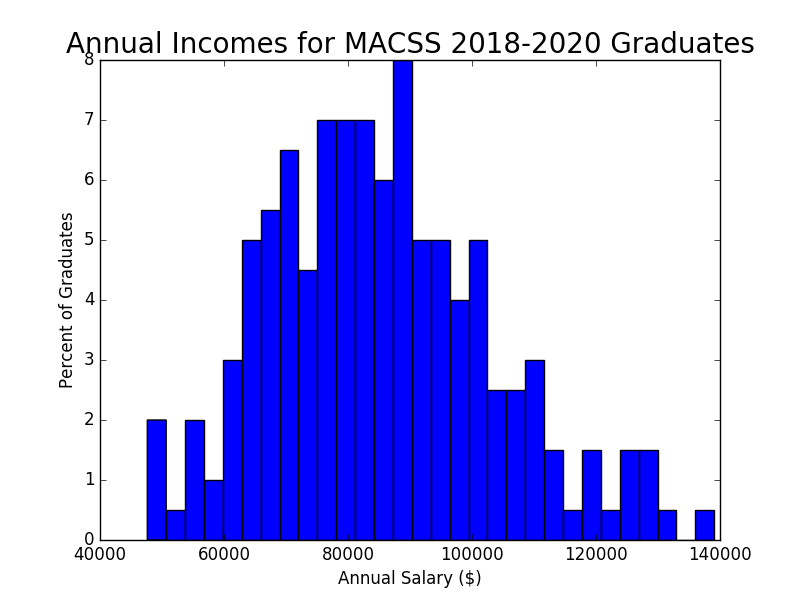
\includegraphics{PS2_1a.png}}}
\end{figure}

\noindent\newline\textbf{Part 1b.} Below is the histogram illustrating the normalized number of MACS 2018-2020 graduates and their annual incomes, generated from the income.txt file. The lognormal probability distribution function with mean ($\mu$) = 9 and standard deviation ($\sigma$) = 0.3 has been plotted in red. This is red line represents the initial "guess" for the $\mu$ and $\sigma$ parameters for our model (in this problem, the model used is the lognormal pdf).

\clearpage

\begin{figure}[htb]\centering\captionsetup{width=4.0in}
  \caption{\textbf{Histogram of Annual Incomes for MACS 2018-2020 Graduates, Normalized}}\label{FigPS2_1b}
  \fbox{\resizebox{4.0in}{3.0in}{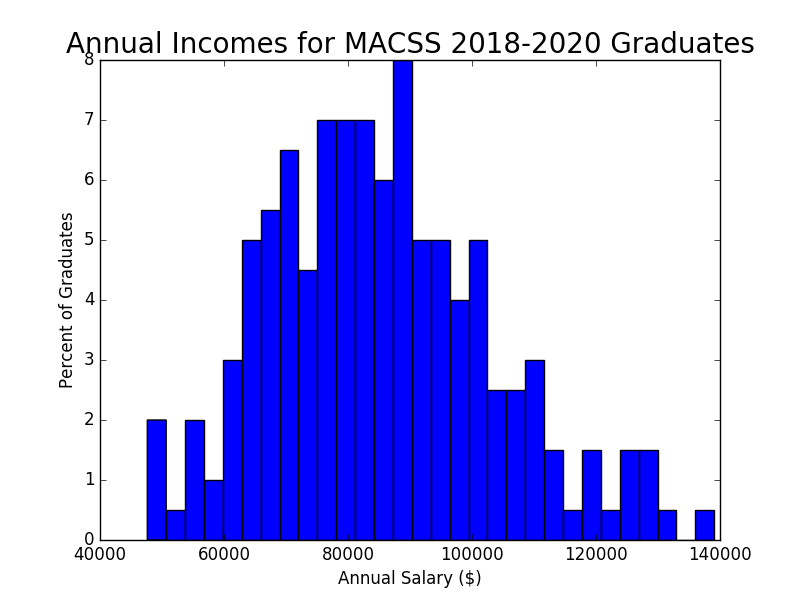
\includegraphics{PS2_1a.png}}}
\end{figure}

\noindent\newline\textbf{Part 1c.} The initial "guess" for the parameters $\mu$ and $\sigma$ were used to estimate the true values of these same parameters using maximum likelihood method. Optimization methods 'TNC', 'L-BFGS-B' and 'SLSQP' were all attempted. Method SLSQP returned what seemed to be the best fit and was the only method to successfully terminate; however, no variance-covariance matrix was returned. Only method TNC returned the inverse hessian. The value of the parameters $\mu$ and $\sigma$  are reported below for both method SLSQP and TNC. The variance-covariance matrix (inverse hessian) has only been provided for method TNC. The estimated parameter values for $\mu$ and $\sigma$ as returned by the MLE method SLSQP has been plotted in green in the histogram below. The value of the log-likehood function using MLE method SLSQP is -2239.53474401.

\clearpage

\begin{figure}[htb]\centering\captionsetup{width=4.0in}
  \caption{\textbf{Histogram of Annual Incomes for MACS 2018-2020 Graduates, Normalized}}\label{FigPS2_1b. Note: for visualization purposes, the normalized number of graduates has been used to generate the histogram. The y-axis scale for the histogram in Part 1a makes it difficult to view any details of the plotted PDF lines. This is contrary to the PS2 directions, which ask for the initial "guess" and estimated MLE PDF lines to be plotted against the histogram from Part 1a. }
  \fbox{\resizebox{4.0in}{3.0in}{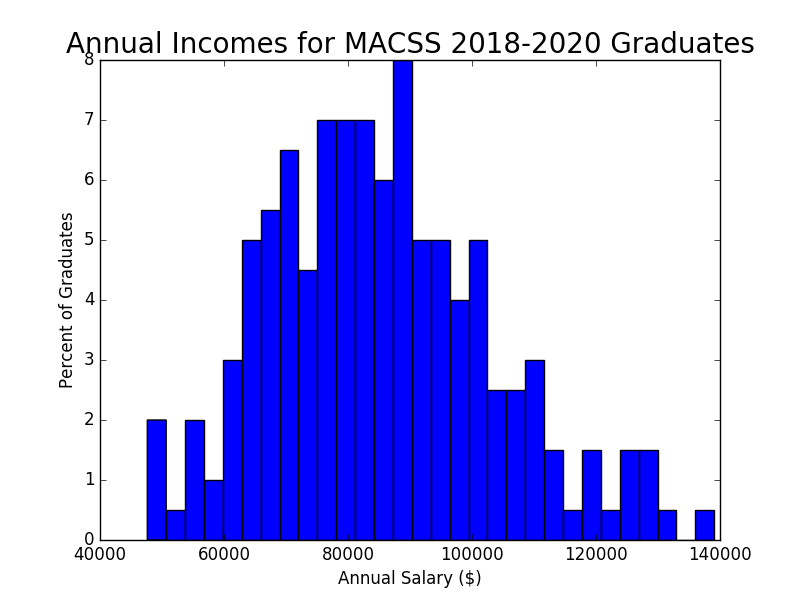
\includegraphics{PS2_1a.png}}}
\end{figure}

\begin{center}
    \caption{MLE method parameter estimates}
    \begin{tabular}{ | l | l | p{5cm} |}
    \hline
    Method & Item & Value  \\ \hline
    SLSQP & $\mu$ & 11.3314417737  \\ \hline
    SLSQP & $\sigma$  & 0.211676166182 \\ \hline
    TNC & $\mu$ & 11.2887517273 \\ \hline
    SLSQP & $\sigma$  & 0.681189027336 \\ \hline
    \end{tabular}
\end{center}

\begin{center}
    \caption{Variance-covariance matrix for method TNC}
    \begin{tabular}{ | p{1cm}| p{1cm} |}
    \hline
    1.0 & 0  \\ \hline
    0 & 1.0 \\ \hline
    \end{tabular}
\end{center}

\noindent\newline\textbf{Part 1d.} The likelihood ration test was performed using outputs from MLE method SLSQP. The chi-squared of H0 with 2 degrees of freedom p-value is 0.0. This tells us that it is unlikely that the data in incomes.txt came from the initial distribution which we "guessed" in part b.

\noindent\newline\textbf{Part 1e.} Using the parameters obtained from MLE method SLSQP in our model, the probability that I will earn greater than \$100,000 per year after graduation is 19.58\%. The probability that I will earn less than \$75,000 per year after graduation is 30.77\%.


\noindent\newline\textbf{Problem 2}
\noindent\newline\textbf{Part 2a.} An initial guess of parameters (taken from part b) $\beta_{0}$ = 1.0, $\beta_{1}$, $\beta_{2}$, $\beta_{3}$ = 0, and $\sigma$  = 0.1 were used to maximze the likelihood of seeing the data in datafile sick.txt.  Optimization methods 'TNC', 'L-BFGS-B' and 'SLSQP' were all attempted. Only method SLSQP terminated successfully, while only Method L-BFGS-B returned the inverse Hessian. The parameter outputs from method SLSQP were input as the initial parameters for Method L-BFGS-B to attempt to improve the optimization. The initial parameters used with Method L-BFGS-B (that is, the outputs from method SLSQP) are reported below, alongside the outputs from the optimization (parameter estimates, variance-covariance matrix). The value of the log-likehood function for this optimization procedure is 0.

\begin{center}
    \caption{MLE method L-BFGS-B parameter estimates}
    \begin{tabular}{ | l | l | l |}
    \hline
    Parameter & Initial Parameter Estimate & Output MLE Parameter estimate \\ \hline
    $\beta_{0}$ & 46.0198488659  & 46.01984887  \\ \hline
    $\beta_{1}$ & 103.89834802 & 103.89834802 \\ \hline
    $\beta_{2}$ & -82.603516994  & -82.60351699 \\ \hline
    $\beta_{3}$ & -83.0455650978  & -83.0455651 \\ \hline
    $\sigma$  & -420.918478405 & -420.91847841 \\ \hline
    \end{tabular}
\end{center}

\begin{center}
    \caption{Variance-covariance matrix for method L-BFGS-B}
    \begin{tabular}{ | p{1cm}| p{1cm}| p{1cm}| p{1cm}| p{1cm}|}
    \hline
    1.0 & 0 & 0 & 0 & 0  \\ \hline
     0 & 1.0 & 0 & 0 & 0  \\ \hline
     0 & 0 & 1.0 & 0 & 0  \\ \hline
     0 & 0 & 0 & 1.0 & 0  \\ \hline
     0 & 0 & 0 & 0 & 1.0  \\ \hline
    \end{tabular}
\end{center}

\noindent\newline\textbf{Part 2b.} A likelihood ratio test was used to determine the probability that our initial guess estimates $\beta_{0}$ = 1.0, $\beta_{1}$, $\beta_{2}$, $\beta_{3}$ = 0, and $\sigma$  = 0.1 fit the model we created using MLE method L-BFGS-B. The chi-squared of H0 with 5 degrees of freedom p-value is 0.0. This tells us that it is unlikely that these parameters are correct: age, number of children, and average winter temperature should have an effect on the number of sick days.

\end{document}

